% Part III: spectral tools (sections 7-8)
\addcontentsline{toc}{part}{Part III \quad Spectral tools}
\section{Fourier analysis: why noise erases fine detail}\label{sec:fourier}

\subsection{Waves}

A complex number is $u+iv$ with $i^2=-1$. Euler's formula $e^{i\theta}=\cos\theta+i\sin\theta$ packs a cosine and a
sine into one exponential of modulus one. The function $x\mapsto e^{ikx}$ is a \emph{wave} of frequency $k$: it
oscillates $k/2\pi$ times per unit length. Large $k$ means fast oscillation, fine detail.

The \emph{Fourier transform} decomposes a function into waves:
\begin{equation}\label{eq:ft}
  \hat f(k)=\int f(x)\,e^{-ikx}\dd x,\qquad f(x)=\frac{1}{2\pi}\int\hat f(k)\,e^{ikx}\dd k .
\end{equation}
$|\hat f(k)|$ says how much of frequency $k$ the function contains. For a density $p$, $\hat p(k)=\E[e^{-ika}]$ is
the \emph{characteristic function}, and its logarithm is the cumulant expansion of \S\ref{sec:cumulants} with
$s=-ik$. On a grid of $N_g$ points the discrete version is computed by the fast Fourier transform (FFT) in
$O(N_g\log N_g)$ operations.

\subsection{Why waves: shifts, convolutions, derivatives}

Waves are special because \emph{shifting a wave only multiplies it by a number}: $e^{ik(x-c)}=e^{-ikc}e^{ikx}$. Three
consequences follow, each in one line.
\begin{itemize}
\item \textbf{Shift.} If $g(x)=f(x-c)$ then $\hat g(k)=e^{-ikc}\hat f(k)$.
\item \textbf{Convolution.} The convolution $(f*g)(x)=\int f(y)g(x-y)\dd y$ is a weighted sum of shifted copies
  of $g$. Substituting $x=y+u$ in $\int\!\!\int f(y)g(x-y)e^{-ikx}\dd y\dd x$ splits it into
  $\int f(y)e^{-iky}\dd y\int g(u)e^{-iku}\dd u$:
  \begin{equation}\label{eq:convthm}
    \widehat{f*g}=\hat f\,\hat g .
  \end{equation}
  Convolution, which costs $O(N_g^2)$ on a grid, becomes multiplication, which costs $O(N_g)$.
\item \textbf{Derivatives.} Integrating by parts, $\widehat{f'}(k)=ik\hat f(k)$, so $\widehat{f''}(k)=-k^2\hat f(k)$. On a grid the
  second difference \eqref{eq:seconddiff} acts on a wave as
  $e^{ik(x+h)}-2e^{ikx}+e^{ik(x-h)}=-4\sin^2(kh/2)\,e^{ikx}$, i.e.\ multiplication by $-\tfrac{4}{h^2}\sin^2(kh/2)\approx-k^2$.
  Waves are the eigenfunctions of the Laplacian, with eigenvalue $-k^2$.
\end{itemize}

\subsection{Noise is a low-pass filter}

The density of a sum of independent quantities is the convolution of their densities. So for the channel
\eqref{eq:channel}, by \eqref{eq:convthm} and the Gaussian transform $\widehat{\N(0,\sigma^2)}(k)=e^{-\sigma^2k^2/2}$
(complete the square in the exponent),
\begin{equation}\label{eq:noisefourier}
  \hat p_t(k)=\hat p_0(\alpha k)\;e^{-\Delta k^2/2}.
\end{equation}
The factor $e^{-\Delta k^2/2}$ crushes high frequencies: sharp features of the clean density, such as two narrow
humps separated by a dip, are the first casualties. Figure~\ref{fig:fourier} shows it on the $\phi^4$ marginal:
its two humps are gone by $t\approx0.3$, and at $t=0.7$ the noised density is visibly a Gaussian.

\begin{figure}[h]\centering
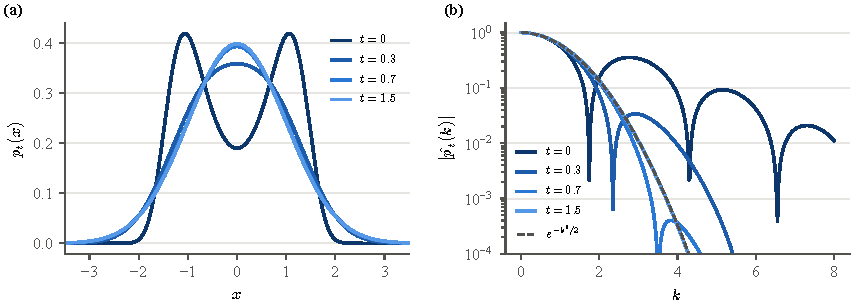
\includegraphics{primer-fourier.pdf}
\caption{(a) The standardised $\phi^4$ marginal at $\Th=0.3$, $h=1$ ($t=0$) and its noised versions. (b) The modulus
of their Fourier transforms. The clean density has strong high-frequency content (the oscillating lobes);
noise multiplies by $e^{-\Delta k^2/2}$ and leaves the Gaussian envelope $e^{-k^2/2}$ (dashed).}
\label{fig:fourier}
\end{figure}

\subsection{The heat equation}

Let $u(x,s)$ evolve by the \emph{heat equation} $\partial_su=\tfrac12\partial_x^2u$: the value at each point moves
towards the average of its neighbours, at a rate set by the second difference. In Fourier variables the
right side is $-\tfrac12k^2\hat u$, so each wave evolves on its own, $\hat u(k,s)=\hat u(k,0)e^{-k^2s/2}$. Comparing with
\eqref{eq:noisefourier}: running the heat equation for time $s$ is the same as convolving with $\N(0,s)$. The
density of a randomly walking particle obeys the heat equation, and ``adding Gaussian noise'' and ``diffusing''
are the same operation. We will meet the heat equation again as the spring term of the Allen--Cahn equation.

\subsection{Fourier and belief propagation}

The $\phi^4$ transfer kernel (\S\ref{sec:transfer}) has the form $T(\phi,\phi')=D(\phi)\,G(\phi'-\phi)\,D(\phi')$, with $G$ a
Gaussian. A message update is then: multiply by $D$ in real space, convolve with $G$ (diagonal in Fourier
space), multiply by $D$ and by the likelihood (diagonal in real space). With FFTs in between, a step costs
$O(N_g\log N_g)$ instead of $O(N_g^2)$. This was the meeting's ``Fourier BP'' idea, and the field makes it natural.
We measured that it cannot pay much at our sizes: at $N_g=401$ the dense product is a minority of the sweep
time, which is dominated by memory traffic, so the end-to-end speed-up is capped near $1.3\times$ (E24). A
truncated Fourier series of a message can also go negative, which a probability cannot.

\begin{caution}
Three spectral ideas must not be confused. \emph{Fourier modes} are a computational basis (diagonalise
convolution). \emph{Hermite modes} (next chapter) diagonalise the noising channel. \emph{Transfer-operator
eigenfunctions} (\S\ref{sec:transfer}) describe the stationary law and the correlation length of the field.
\end{caution}

\paragraph{Check yourself.}
\begin{enumerate}[label=\thesection.\arabic*,leftmargin=2.2em]
\item Why does adding independent noise $\sqrt\Delta z$ multiply the characteristic function by $e^{-\Delta k^2/2}$?
\item On a grid of spacing $h$, the fastest wave has wavelength $2h$ ($k=\pi/h$). By what factor does the second
  difference multiply it?
\end{enumerate}

\section{Hermite polynomials: why fourth-order structure fades like $e^{-4t}$}\label{sec:hermite}

\subsection{The right basis for the channel}

The channel \eqref{eq:channel} does two things: it shrinks ($a\mapsto e^{-t}a$) and it blurs (adds Gaussian noise).
Waves diagonalise blurring but not shrinking. Polynomials orthogonal with respect to the Gaussian
diagonalise both. Define the inner product $\langle f,g\rangle=\E[f(Z)g(Z)]$ for $Z\sim\N(0,1)$ and orthogonalise
$1,x,x^2,\dots$ one at a time (Gram--Schmidt). Using $\E Z^2=1$, $\E Z^4=3$, $\E Z^6=15$:
\begin{equation}\label{eq:hermite}
  H_0=1,\quad H_1=x,\quad H_2=x^2-1,\quad H_3=x^3-3x,\quad H_4=x^4-6x^2+3,\ \dots
\end{equation}
For instance $H_2=x^2-\E Z^2$ removes the part of $x^2$ along $1$, and $H_3=x^3-3x$ removes the part along
$x$ ($\E[Z^3\cdot Z]=3$). These are the (probabilists') \emph{Hermite polynomials} (Figure~\ref{fig:hermite}a). They
have a compact \emph{generating function},
\begin{equation}\label{eq:genfun}
  G(x;s)=e^{sx-s^2/2}=\sum_{n\ge0}H_n(x)\frac{s^n}{n!},
\end{equation}
from which everything follows. Orthogonality: $\E[G(Z;s)G(Z;r)]=e^{-(s^2+r^2)/2}\E e^{(s+r)Z}=e^{sr}$, and matching
powers of $sr$ gives $\E[H_mH_n]=n!$ if $m=n$ and $0$ otherwise. Differentiating \eqref{eq:genfun} in $x$ gives
$H_n'=nH_{n-1}$.

\subsection{The channel multiplies $H_n$ by $e^{-nt}$}

\begin{proposition}\label{prop:hermite}
For $f$ a function, let $(P_tf)(a)=\E\big[f(e^{-t}a+\sqrt{1-e^{-2t}}\,Z)\big]$ be the average of $f$ over the channel
started at $a$. Then $P_tH_n=e^{-nt}H_n$.
\end{proposition}
\begin{proof}
Apply $P_t$ to the generating function. With $\alpha=e^{-t}$, $\Delta=1-\alpha^2$,
\[
  P_tG(\cdot;s)(a)=\E\,e^{s\alpha a+s\sqrt\Delta Z-s^2/2}=e^{s\alpha a+s^2\Delta/2-s^2/2}=e^{(s\alpha)a-(s\alpha)^2/2}=G(a;s\alpha),
\]
because $\Delta-1=-\alpha^2$. Expanding both sides in powers of $s$: $\sum_n(P_tH_n)(a)s^n/n!=\sum_nH_n(a)\alpha^ns^n/n!$.
\end{proof}

\subsection{Densities, cumulants, and the noised law}

Write a standardised density relative to the Gaussian as
\begin{equation}\label{eq:gramcharlier}
  p(a)=\varphi(a)\Big(1+\sum_{n\ge3}c_n\frac{H_n(a)}{n!}\Big),\qquad c_n=\E_p[H_n(a)],
\end{equation}
with $\varphi$ the standard normal density; the coefficients are read off by orthogonality, and $c_1=c_2=0$ because
the law is standardised. In particular $c_3=\E a^3$ is the skewness and $c_4=\E a^4-3$ the excess kurtosis. Now
noise it. The noised quantity $x$ has $\E[H_n(x)]=\E[(P_tH_n)(a)]=e^{-nt}c_n$ by Proposition~\ref{prop:hermite}, so
\begin{equation}\label{eq:noisedgc}
  p_t(x)=\varphi(x)\Big(1+\sum_{n\ge3}c_n\,e^{-nt}\,\frac{H_n(x)}{n!}\Big).
\end{equation}
\begin{keyidea}
The channel leaves the Gaussian part alone and multiplies the $n$-th Hermite coefficient by $e^{-nt}$. Mean
information decays like $e^{-t}$, covariance like $e^{-2t}$, skewness like $e^{-3t}$, kurtosis like $e^{-4t}$
(Figure~\ref{fig:hermite}b). Fourth-order distinctions vanish under noise long before second-order ones.
\end{keyidea}

\begin{figure}[h]\centering
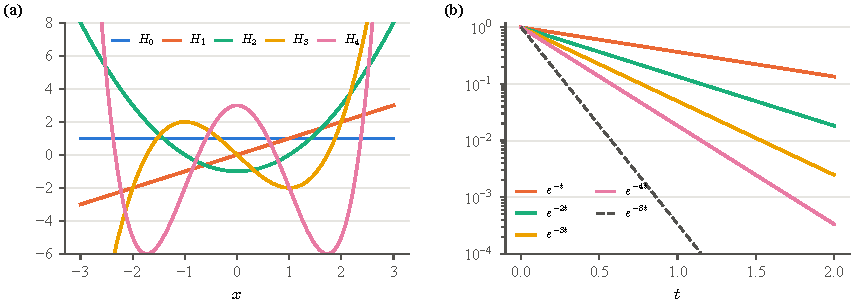
\includegraphics{primer-hermite.pdf}
\caption{(a) The Hermite polynomials $H_0,\dots,H_4$. (b) The factors $e^{-nt}$ by which the channel multiplies their
coefficients, and $e^{-8t}$, the decay of the squared non-Gaussian part of the score.}
\label{fig:hermite}
\end{figure}

\subsection{What a Gaussian denoiser misses: Theorem 2 at one site}

Take a symmetric law ($c_3=0$) and the score of \eqref{eq:noisedgc}. To first order in the small correction,
$\log p_t=\log\varphi+\log(1+R)\approx-x^2/2+R$, so using $H_n'=nH_{n-1}$,
\begin{equation}\label{eq:scorehermite}
  s_t(x)\approx-x+\sum_{n\ge3}c_n\,e^{-nt}\frac{H_{n-1}(x)}{(n-1)!}=-x+\frac{\kappa_4\,e^{-4t}}{6}\,H_3(x)+O(e^{-6t}).
\end{equation}
The covariance twin's score is exactly $-x$. Their mean-square distance is therefore
\[
  \E\big[(s_t-s_t^{\rm G})^2\big]\approx\frac{\kappa_4^2e^{-8t}}{36}\,\E[H_3^2]=\frac{\kappa_4^2}{6}\,e^{-8t}.
\]
This is the single-site version of the paper's Theorem~2, which states for a whole chain that the gap
between the exact score and the Gaussian (closure) score behaves like $\tfrac16\|\kappa_4\|_F^2e^{-8t}$, with
$\kappa_4$ the tensor of fourth cumulants across sites. On the $\phi^4$ field the ratio of the measured gap to this
prediction rises towards one with $t$ and reaches $0.73$ to $0.94$ at $t=3$ (E32, frozen).

\subsection{Many sites}

For a sequence, use products $H_{n_1}(x_1)\cdots H_{n_L}(x_L)$. The same proof shows that the channel multiplies
such a product by $e^{-(n_1+\dots+n_L)t}$. The covariance between sites $i$ and $j$ is the coefficient of
$H_1(x_i)H_1(x_j)$, degree $2$, so it survives like $e^{-2t}$; a fourth cumulant across sites has total degree
$4$ and fades like $e^{-4t}$.

\begin{caution}
Adding independent Gaussian noise $\sigma z$ to $a$ does \emph{not} change its cumulants of order $3$ and higher
(they add, and the Gaussian contributes zero). What shrinks is their size \emph{relative to the variance},
which grows. Under the variance-preserving channel the two effects are combined into the single factor
$\alpha^n=e^{-nt}$ of \eqref{eq:cumdecay}. Both descriptions say the same thing; mixing them up is a common
source of wrong exponents.
\end{caution}

\paragraph{Check yourself.}
\begin{enumerate}[label=\thesection.\arabic*,leftmargin=2.2em]
\item Check directly that $H_3$ is orthogonal to $H_1$ under the standard normal.
\item By what factor does the non-Gaussian part of the score in \eqref{eq:scorehermite} shrink between $t=0.5$ and $t=1$?
  And its squared error?
\end{enumerate}
